\documentclass[12pt,a4paper]{report}

\usepackage{graphicx}
\usepackage{amsmath,amssymb}
\usepackage{geometry}
\usepackage{setspace}
\usepackage{lmodern}
\usepackage{hyperref}
\usepackage{float}
\usepackage{placeins}
\usepackage{tikz}

\usetikzlibrary{
    arrows.meta,
    positioning,
    fit,
    backgrounds
}

\graphicspath{{images/}}
\geometry{margin=1in}
\setstretch{1.2}

\begin{document}

% ================== TITLE PAGE ==================
\begin{titlepage}
\centering

{\LARGE \textbf{AI Virtual Coach} \\[1em]}
{A Bachelor's Graduation Project} \\[1.5em]

\includegraphics[width=1\linewidth]{E-JUST_logo.png} \\[2em]
\begin{figure}
    \centering
    \label{fig:placeholder}
\end{figure}
{\Large \textsc{EGYPT-JAPAN UNIVERSITY FOR SCIENCE AND TECHNOLOGY}} \\[0.5em]
{\large \textsc{FACULTY OF ENGINEERING}} \\[1em]
{\normalsize \textsc{DEPARTMENT OF COMPUTER SCIENCE AND ENGINEERING}} \\[2em]

{\Large \textbf{Ahmed Mohamed Ahmed Ali}} \\
Student ID: 120220150 \\[1em]

{\Large \textbf{Zeyad Mohamed Mahmoud}} \\
Student ID: 120210333 \\[1em]

{\Large \textbf{Al Amir Hossam}} \\
Student ID: 120210301 \\[2em]

Supervisor: \textbf{Prof. Walid Gomaa} \\[2em]

\begin{itshape}
This thesis was presented as a partial fulfillment of the requirements for the Bachelor of Engineering in Computer Science.
\end{itshape}

\vfill
\textbf{February 2026}

\end{titlepage}

% ================== FRONT MATTER ==================
\chapter*{Acknowledgements}
The authors would like to express their sincere gratitude to their supervisor, Dr. Walid Gomaa, for his continuous guidance, constructive feedback, and valuable support throughout the development of this project. His expertise and encouragement were instrumental in shaping the direction of this work.

The authors would also like to thank their teammates for their collaboration, discussions, and shared efforts during all stages of the project. Appreciation is extended to the Egypt-Japan University of Science and Technology and the Faculty of Engineering for providing the academic environment and resources necessary to complete this work.

Finally, the authors acknowledge the research papers and prior studies that inspired and informed this project. These works provided essential theoretical foundations and practical insights that contributed significantly to the development of the proposed system.

\chapter*{Abstract}
Resistance training exercises are characterized by structured and repeatable movement patterns, making them well-suited for computational analysis and automated coaching. However, improper exercise execution remains a common issue due to limited access to professional supervision. This thesis presents a vision-based AI virtual coaching system designed to analyze resistance training exercises using consumer-grade RGB video.

The proposed system integrates three core models: exercise recognition, exercise quality assessment, and gender recognition. Human pose estimation is first applied to extract biomechanical features from video recordings captured under realistic gym conditions. The exercise recognition model identifies the performed movement among 15 resistance training exercises, while the assessment model evaluates execution quality using multiple predefined biomechanical aspects annotated by certified fitness coaches. A repetition-aware framework is employed to handle the cyclic nature of resistance training movements despite coarse set-level supervision.

The system is evaluated using subject-disjoint experimental protocols to assess generalization to unseen users. Experimental results demonstrate that pose-based representations combined with lightweight machine learning models can achieve reliable exercise recognition and meaningful quality assessment without requiring wearable sensors or specialized hardware.

These findings highlight the potential of vision-based virtual coaching systems as scalable, accessible alternatives to traditional in-person fitness supervision.

\tableofcontents
\listoffigures
\listoftables
\clearpage

% ================== CHAPTER 1 ==================
\chapter{Introduction}

\section{Motivation and Problem Statement}
Resistance training is one of the most widely practiced forms of physical activity due to its proven benefits in improving muscular strength, endurance, metabolic health, and overall physical well-being. Unlike many forms of free-form physical activity, resistance training exercises consist of structured and repeatable movement patterns, making them particularly suitable for computational analysis. These properties allow reliable extraction of biomechanical features and enable systematic evaluation of exercise execution quality.

Despite its benefits, improper execution of resistance training exercises remains a significant concern. Incorrect form can reduce training effectiveness and substantially increase the risk of acute and chronic musculoskeletal injuries. Traditionally, correct execution is ensured through supervision by qualified fitness coaches or physiotherapists. However, continuous professional supervision is often expensive, time-consuming, and inaccessible to a large portion of the population. As a result, many individuals train without expert guidance, relying instead on mirrors, prerecorded instructional videos, or informal advice, none of which provide personalized, real-time feedback.

The growing demand for scalable fitness solutions has motivated the development of virtual coaching systems capable of providing automated exercise analysis and feedback. Advances in artificial intelligence and computer vision have made it feasible to analyze human movement directly from video data. In particular, recent progress in human pose estimation enables accurate extraction of biomechanical information using standard RGB cameras, without the need for specialized hardware.

A vision-based approach was selected in this work due to its non-intrusive nature, cost-effectiveness, and ease of deployment. Unlike wearable sensor–based systems, camera-based solutions do not require users to attach, charge, or calibrate devices, which improves usability and reduces setup errors. Low user compliance is a common limitation of wearable-based systems, as sensors are often forgotten, misplaced, or worn incorrectly. By relying solely on video input, the proposed system removes this dependency while still enabling detailed movement and body analysis.

Furthermore, vision-based systems are highly scalable, as they can be deployed using existing cameras in gyms or smartphones in home environments. This enables the development of accessible virtual coaching solutions that operate under realistic conditions without additional hardware costs. However, designing such systems presents several challenges, including handling inter-subject variability, operating under unconstrained recording conditions, and moving beyond simple exercise recognition toward meaningful assessment of execution quality.

This thesis addresses these challenges by proposing an AI-based virtual coaching system that leverages pose estimation and machine learning to analyze resistance training exercises from RGB video, providing both exercise recognition and execution quality assessment.

\section{Objectives of the Thesis}
The primary objective of this thesis is to design, implement, and evaluate an intelligent virtual coaching system capable of analyzing resistance training exercises using computer vision techniques.

To achieve this goal, the thesis focuses on the following specific objectives:
\begin{itemize}
    \item Develop an exercise recognition model that accurately identifies resistance training exercises performed by a user from video input.
    \item Design an exercise assessment model that evaluates execution quality using multiple biomechanical aspects, reflecting how human coaches assess exercise performance.
    \item Implement a gender recognition model to support user characterization and analysis within the virtual coaching framework.
    \item Construct a complete end-to-end pipeline that integrates pose estimation, feature extraction, recognition, assessment, and feedback generation.
    \item Evaluate the proposed system under subject-disjoint experimental protocols to assess generalization to unseen users.
\end{itemize}

\section{Contributions}
The main contributions of this thesis can be summarized as follows:
\begin{itemize}
    \item The collection of a real-world dataset comprising resistance training exercises performed by 51 participants and recorded from front and side viewpoints using smartphone cameras.
    \item The design of an interpretable, pose-based feature representation tailored to resistance training movements.
    \item The development of a subject-independent exercise recognition model supporting 15 resistance training exercises.
    \item The proposal of a repetition-aware exercise assessment framework that predicts multiple biomechanical quality aspects rather than a single scalar score.
    \item The design of a hybrid coaching feedback agent combining deterministic rule-based analysis with large language model generation, enabling personalized natural language coaching feedback grounded in per-repetition assessment data.
    \item The integration of recognition, assessment, and coaching models into a unified virtual coaching architecture capable of generating actionable feedback.
\end{itemize}

\section{Thesis Organization}
The remainder of this thesis is organized as follows. Chapter~2 presents background concepts and a review of related work in pose estimation, human action recognition, and action quality assessment. Chapter~3 describes the dataset, data collection process, annotation protocol, and dataset limitations. Chapter~4 introduces the overall system architecture and feature engineering methodology. Chapter~5 details the exercise recognition model, including its formulation, architecture, and evaluation. Chapter~6 presents the exercise assessment framework and repetition-aware modeling approach. Chapter~7 describes the gender recognition model and its role within the system. Chapter~8 presents the coaching agent module, which translates numerical assessment outputs into personalized natural language feedback using a hybrid deterministic and large language model architecture. Chapter~9 reports experimental results and provides performance analysis. Finally, Chapter~10 concludes the thesis and outlines limitations and directions for future work.

\chapter{Background and Literature Review}

This chapter reviews the key research areas related to the proposed AI Virtual Coach. The discussion covers human pose estimation, exercise and action recognition, action quality assessment, and AI-based virtual coaching systems. The purpose of this review is to position the proposed work within the existing literature and to highlight the research gaps addressed by this thesis.

\section{Human Pose Estimation}

Human pose estimation is the task of localizing anatomical keypoints of the human body from images or video sequences. These keypoints, typically representing joints and body landmarks, form a skeletal representation that captures the spatial configuration of the human body. Pose estimation serves as a foundational component for many higher-level tasks, including action recognition, motion analysis, and human–computer interaction.

Early approaches to pose estimation relied on graphical models and handcrafted features, such as pictorial structures and part-based models. While these methods provided interpretable formulations, they were limited in robustness and computational efficiency. Recent advances in deep learning have significantly improved pose estimation accuracy by enabling end-to-end learning from large-scale datasets.

Modern pose estimation frameworks include OpenPose, AlphaPose, and MediaPipe Pose. These systems use convolutional neural networks to directly regress joint locations from RGB input. MediaPipe Pose, in particular, is designed for real-time performance on consumer-grade hardware and provides 33 body landmarks per frame. It operates on monocular RGB video and does not require depth sensors or multi-camera setups, making it well suited for practical applications.

In this thesis, MediaPipe Pose is employed to extract 2D pose landmarks from RGB video. Pose-based representations offer several advantages over raw video, including reduced sensitivity to background appearance, lighting conditions, and clothing variations. Additionally, skeletal representations preserve biomechanical interpretability, which is essential for analyzing exercise execution quality.

\section{Exercise and Action Recognition}

Human action recognition aims to identify the type of activity being performed by an individual based on visual input. Traditional action recognition methods relied on handcrafted spatio-temporal features such as optical flow, trajectory descriptors, and motion histograms. Techniques such as Hidden Markov Models and Dynamic Time Warping were commonly used to model temporal dynamics in early systems.

With the rise of deep learning, convolutional neural networks became the dominant paradigm for action recognition. Two-stream architectures process spatial appearance and temporal motion separately, while three-dimensional CNNs extend convolution operations into the temporal dimension. More recently, recurrent neural networks and transformer-based architectures have been proposed to model long-range temporal dependencies.

Despite their strong performance, many deep learning approaches require large-scale labeled datasets and substantial computational resources. This limits their applicability in domains such as fitness analysis, where datasets are relatively small and deployment constraints favor lightweight models.

Pose-based action recognition has emerged as an effective alternative that balances performance and efficiency. By operating on skeletal data rather than raw pixels, pose-based methods reduce dimensionality and focus on motion dynamics. Such approaches have demonstrated competitive performance while remaining more interpretable and data-efficient. In the context of resistance training, pose-based representations are particularly suitable due to the structured and repetitive nature of exercises.

\section{Action Quality Assessment}

Action Quality Assessment (AQA) extends beyond recognizing an action category to evaluating how well the action is performed. Unlike action recognition, which produces a discrete label, AQA typically involves regression or ranking to estimate execution quality or skill level.

Early AQA research focused on sports domains such as diving, gymnastics, and figure skating, where performances are scored by judges. These methods often predict a single scalar score for an entire video sequence and rely on either handcrafted features or deep temporal models. Recent work has explored relative ranking approaches and contrastive learning to handle annotation noise and subjectivity.

Applying AQA to fitness and resistance training presents unique challenges. Resistance training exercises consist of repeated motion cycles, and execution quality may vary across repetitions within a single set. Furthermore, human coaches typically assess multiple biomechanical aspects, such as joint alignment, range of motion, stability, and movement control, rather than relying on a single overall score.

Another challenge is annotation granularity. In many fitness datasets, expert annotations are provided at the exercise-set level rather than at the individual repetition level. This mismatch between input granularity and supervision complicates model design and training. Addressing these challenges motivates the repetition-aware, multi-aspect assessment framework proposed in this thesis.

\section{AI-Based Virtual Coaching Systems}

AI-based virtual coaching systems aim to provide automated guidance, feedback, and performance analysis for physical activities. Early systems focused on rule-based feedback or simple pose visualization, offering limited personalization. Advances in computer vision and machine learning have enabled more sophisticated systems capable of recognizing exercises, detecting errors, and providing corrective feedback.

Recent virtual coaching applications often combine pose estimation with machine learning models to analyze user movements from video. Mobile applications, in particular, have gained popularity due to the widespread availability of smartphones with high-quality cameras. These systems prioritize ease of use, real-time performance, and minimal hardware requirements.

Some virtual coaching systems integrate multimodal sensors such as inertial measurement units or depth cameras to improve accuracy. However, these approaches increase system complexity and reduce accessibility. Vision-based systems that rely solely on RGB video offer a more scalable alternative, especially when combined with robust pose estimation techniques.

More advanced systems incorporate feedback mechanisms that translate numerical analysis into human-readable guidance. This includes textual feedback, visual cues, or conversational interfaces. Such systems benefit from separating low-level motion analysis from high-level feedback generation, enabling modular design and improved interpretability.

The system proposed in this thesis follows this design philosophy by combining pose-based recognition and assessment with a feedback-oriented virtual coaching framework suitable for deployment in real-world gym and home environments.

\section{Summary and Research Gap}

The reviewed literature demonstrates significant progress in pose estimation, action recognition, and action quality assessment. However, several gaps remain in the context of resistance training and practical virtual coaching. Existing approaches often focus on recognition rather than quality assessment, rely on single-score evaluation, or require specialized hardware and large datasets.

This thesis addresses these gaps by proposing a lightweight, pose-based virtual coaching system that performs exercise recognition and multi-aspect quality assessment using consumer-grade RGB video. By explicitly modeling repetitions and operating under realistic recording conditions, the proposed approach advances toward accessible and deployable AI-driven fitness coaching solutions.
\chapter{Dataset and Data Collection}

This chapter describes the dataset collected for this thesis and the data acquisition procedures followed during recording and annotation. The dataset was designed to reflect realistic resistance training scenarios while remaining compatible with consumer-grade hardware and practical deployment constraints.

\section{Dataset Overview}

To support the development and evaluation of the proposed AI virtual coaching system, a dedicated dataset of resistance training exercises was collected. The dataset consists of RGB video recordings captured using smartphone cameras under real-world gym conditions.

The dataset includes recordings from 51 participants performing 15 resistance training exercises. Each exercise was recorded from two viewpoints, namely front view and side view, to capture complementary biomechanical information. The dataset supports both exercise recognition and exercise quality assessment tasks.

\section{Participants}

The dataset was collected from a total of 51 recreationally active volunteers, including 41 males (80.4\%) and 10 females (19.6\%). Participant ages ranged from 15 to 29 years, with a mean age of 21.3 years. All participants reported no current musculoskeletal injuries at the time of recording.

The observed gender imbalance reflects practical and cultural constraints associated with video-based data collection in public gym environments in Egypt, where some female gym members preferred not to be recorded. Participation was entirely voluntary, and verbal informed consent was obtained from all participants prior to recording.

To preserve privacy, all data were anonymized using numerical identifiers, and only aggregated demographic statistics are reported.
\begin{table}[h]
\centering
\caption{Gender Distribution of Participants}
\label{tab:gender_distribution}
\begin{tabular}{lcc}
\hline
\textbf{Gender} & \textbf{Number of Participants} & \textbf{Percentage} \\
\hline
Male   & 41 & 80.4\% \\
Female & 10 & 19.6\% \\
\hline
\textbf{Total} & \textbf{51} & \textbf{100\%} \\
\hline
\end{tabular}
\end{table}

\begin{figure}
    \centering
    \includegraphics[width=0.5\linewidth]{GENDER.jpg}
    \caption{Gender Distribution of Participants}
    \label{fig:placeholder}
\end{figure}
\begin{figure}
    \centering
    \includegraphics[width=0.5\linewidth]{age.jpg}
    \caption{Age Distribution of Participants}
    \label{fig:placeholder}
\end{figure}
\begin{figure}
    \centering
    \includegraphics[width=0.5\linewidth]{height.jpg}
    \caption{Height Distribution of Participants}
    \label{fig:placeholder}
\end{figure}
\begin{figure}
    \centering
    \includegraphics[width=0.5\linewidth]{weight.jpg}
    \caption{Weight Distribution of Participants}
    \label{fig:placeholder}
\end{figure}
\begin{figure}
    \centering
    \includegraphics[width=0.5\linewidth]{BMI.jpg}
    \caption{BMI Distribution of Participants}
    \label{fig:placeholder}
\end{figure}
\FloatBarrier

Table~\ref{tab:demographics} summarizes the anthropometric characteristics of the 51 participants.

\begin{table}[h]
\centering
\caption{Participant Anthropometric Summary}
\label{tab:demographics}
\begin{tabular}{lcccc}
\hline
\textbf{Attribute} & \textbf{Min} & \textbf{Max} & \textbf{Mean} & \textbf{SD} \\
\hline
Age (years) & 15 & 29 & 21.3 & 3.1 \\
Height (cm) & 158 & 190 & 174.2 & 7.6 \\
Weight (kg) & 52 & 110 & 77.5 & 13.9 \\
BMI (kg/m$^2$) & 18 & 37 & 24.7 & 4.1 \\
\hline
\end{tabular}
\end{table}

\section{Exercise Set}
The dataset includes recordings of the following 15 resistance training exercises:
\begin{itemize}
    \item Dumbbell Shoulder Press
    \item Hammer Curls
    \item Standing Dumbbell Front Raises
    \item Lateral Raises
    \item Bulgarian Split Squat
    \item EZ-Bar Curls
    \item Incline Dumbbell Bench Press
    \item Overhead Triceps Extension
    \item Shrugs
    \item Weighted Squats
    \item Seated Biceps Curls
    \item Triceps Kickbacks
    \item Rows
    \item Deadlift
    \item Calf Raises
\end{itemize}

These exercises were selected to cover a diverse range of movement patterns, including pushing, pulling, hinging, squatting, and isolation movements. While the dataset includes a larger variety of upper-body exercises than lower-body exercises, the number of participants contributing to each exercise was approximately comparable across both categories.
\begin{table}[h]
\centering
\caption{Body Exercises and Muscle Focus}
\label{tab:exercise_muscle_focus}
\begin{tabular}{ll}
\hline
\textbf{Exercise} & \textbf{Primary Muscle Focus} \\
\hline
Dumbbell Shoulder Press & Deltoids, Triceps \\
Standing Dumbbell Front Raises & Anterior Deltoid \\
Lateral Raises & Lateral Deltoid \\
Shrugs & Trapezius \\
Inclined Dumbbell Bench Press & Upper Chest, Triceps \\
Rows & Lats, Rhomboids, Rear Deltoids \\
EZ-Bar Curls & Biceps \\
Seated Biceps Curls & Biceps (Isolated) \\
Hammer Curls & Biceps, Brachialis \\
Triceps Kickbacks & Triceps \\
Overhead Triceps Extension & Triceps (Long Head) \\
Bulgarian Split Squat & Quadriceps, Glutes, Balance \\
Weighted Squats & Quadriceps, Glutes, Core Stabilization \\
Calf Raises & Gastrocnemius, Soleus \\
Deadlift & Glutes, Hamstrings, Lower Back \\
\hline
\end{tabular}
\end{table}

\section{Recording Setup}

All recordings were conducted indoors at multiple gym facilities in Egypt. Videos were captured using smartphone RGB cameras at a resolution of 1080~$\times$~1920 pixels and a frame rate of 30 frames per second in landscape orientation. Lighting conditions varied across recording sessions, resulting in mixed indoor illumination.

Camera placement was not strictly fixed to emulate realistic user behavior. Depending on the exercise, recordings captured either the full body or were positioned at approximately waist level. Camera distance varied across recordings and was not explicitly constrained.

\section{Recording Protocol}

Each video corresponds to a single exercise set lasting approximately 30 to 60 seconds and containing 8 to 12 repetitions. Videos were recorded as continuous sequences without rest intervals.

Participants performed exercises using self-selected weights to reflect natural training conditions. Exercise execution was not artificially constrained, allowing natural variability in tempo, range of motion, and movement quality. This variability is essential for training and evaluating exercise assessment models.

\section{Viewpoint Acquisition}

To capture complementary kinematic information, each exercise was recorded from two viewpoints:
\begin{itemize}
    \item \textbf{Front view}, capturing bilateral symmetry and lateral movement patterns.
    \item \textbf{Side view}, capturing sagittal-plane dynamics such as joint flexion and torso inclination.
\end{itemize}

A total of 154 videos were recorded per viewpoint, resulting in 308 videos overall. Viewpoints were manually labeled during preprocessing to ensure correct association during analysis.

\section{Annotation Protocol}

Exercise quality annotations were provided by two certified fitness coaches. Annotations were performed at the exercise-set (video) level rather than at the individual repetition level. For each exercise, coaches evaluated five predefined biomechanical aspects tailored to the specific movement, such as joint alignment, range of motion, stability, and movement control.

To combine expert opinions, a reliability-weighted fusion strategy was employed:
\begin{equation}
y = 0.25\,y_{C1} + 0.75\,y_{C2},
\end{equation}
where $y_{C1}$ and $y_{C2}$ denote the scores provided by Coach 1 and Coach 2, respectively. Scores were defined on a 0--10 scale.

Repetition-level clips extracted from each video inherit the corresponding set-level annotation, enabling repetition-aware modeling despite coarse supervision.

Table~\ref{tab:annotation_criteria} provides examples of the assessment criteria defined for representative exercises. Each exercise has five criteria tailored to its specific biomechanical requirements.

\begin{table}[H]
\centering
\caption{Assessment criteria examples for representative exercises. Each exercise is evaluated across five biomechanical aspects defined in consultation with certified fitness coaches.}
\label{tab:annotation_criteria}
\begin{tabular}{p{3.5cm}p{10cm}}
\hline
\textbf{Exercise} & \textbf{Assessment Criteria} \\
\hline
Dumbbell Shoulder Press & (1) Starting position and grip, (2) Pressing path and elbow position, (3) Top position and lockout, (4) Lowering phase and control, (5) Core stability and posture \\
\hline
Weighted Squats & (1) Starting position and stance, (2) Descent phase and depth, (3) Knee tracking and alignment, (4) Ascent phase and drive, (5) Core stability and posture \\
\hline
Deadlift & (1) Starting position and setup, (2) Lifting phase and bar path, (3) Hip hinge and back position, (4) Lockout position, (5) Lowering phase and control \\
\hline
Hammer Curls & (1) Elbow position fixed close to torso, (2) Wrist orientation in neutral grip, (3) Movement control without swinging, (4) Full range of motion, (5) Controlled tempo \\
\hline
\end{tabular}
\end{table}

\section{Pose Extraction and Preprocessing}

For each video, 2D human pose landmarks were extracted using the MediaPipe Pose framework. The model produces 33 body landmarks per frame, forming temporal pose sequences for each exercise.

To reduce variability caused by camera distance and subject body size, landmark coordinates were normalized using a torso-based normalization strategy. Specifically, landmark positions were centered at the hip midpoint and scaled by the distance between the hip and shoulder midpoints. This normalization improves consistency across participants and recording conditions.

\section{Dataset Limitations}

Despite its strengths, the dataset exhibits several limitations. First, the dataset shows a gender imbalance, primarily due to cultural and logistical constraints during data collection. Second, the number of lower-body exercise types is smaller than that of upper-body exercises. Third, recording conditions such as camera placement and lighting were not controlled, which may introduce noise into pose estimation.

Nevertheless, these limitations also reflect realistic deployment conditions. The dataset captures substantial inter-subject variability and natural execution patterns, making it suitable for evaluating the robustness and practical applicability of virtual coaching systems.

\section{Chapter Summary}

This chapter presented the dataset used in this thesis, including participant demographics, exercise selection, recording procedures, annotation protocol, and dataset limitations. The next chapter introduces the overall system architecture and the feature engineering methodology used to transform raw pose data into discriminative representations.
\chapter{System Architecture}

This chapter presents the overall architecture of the proposed AI Virtual Coach. The system is designed as a modular pipeline that processes RGB video input and produces structured exercise analysis and feedback. The architecture integrates pose estimation, feature extraction, exercise recognition, exercise quality assessment, and gender recognition into a unified framework suitable for real-world deployment.

\section{System Overview}

The proposed system follows a multi-stage processing pipeline that transforms raw video input into high-level semantic information. Figure~\ref{fig:system_pipeline} illustrates the overall architecture of the AI Virtual Coach.

The system consists of the following main components:
\begin{itemize}
    \item Video acquisition and preprocessing,
    \item Human pose estimation,
    \item Pose normalization and feature extraction,
    \item Exercise recognition model,
    \item Exercise assessment model,
    \item Gender recognition model,
    \item Feedback and analysis layer.
\end{itemize}

This modular design allows each component to be developed, evaluated, and optimized independently while maintaining end-to-end coherence.

\begin{figure*}[h]
\centering
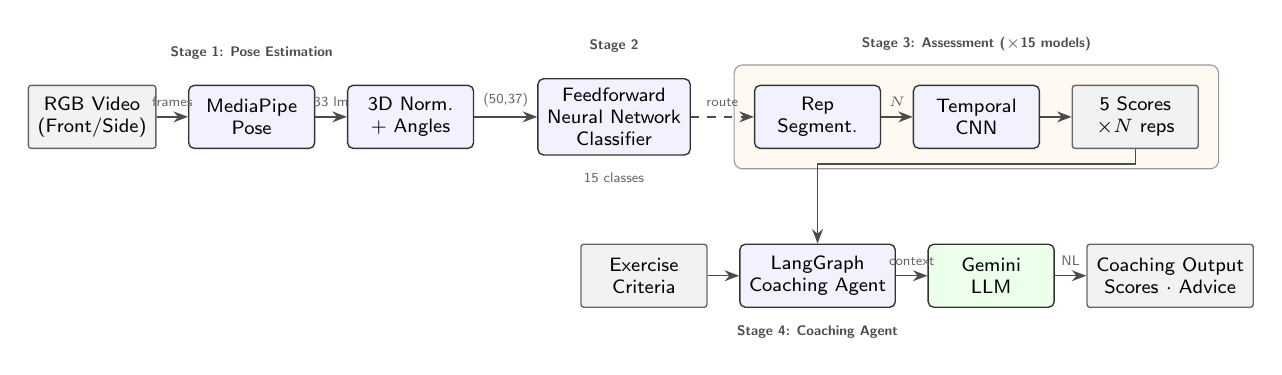
\begin{tikzpicture}[scale=1, transform shape,
    font=\sffamily\scriptsize,
    node distance=4mm,
    box/.style={
        rectangle,
        rounded corners=2pt,
        draw=black!80,
        fill=blue!5,
        line width=0.5pt,
        align=center,
        minimum height=8mm,
        minimum width=16mm
    },
    data/.style={
        rectangle,
        rounded corners=1pt,
        draw=black!60,
        fill=gray!10,
        line width=0.5pt,
        align=center,
        minimum height=8mm,
        minimum width=16mm
    },
    stage/.style={
        font=\sffamily\tiny\bfseries,
        text=black!70
    },
    annot/.style={
        font=\sffamily\tiny,
        text=black!60
    },
    arrow/.style={->, >=Stealth, line width=0.5pt, black!70},
    dashedarrow/.style={->, >=Stealth, dashed, line width=0.5pt, black!70}
]

% ===== ROW 1: Stages 1-3 =====
\node[data] (rgb) {RGB Video\\(Front/Side)};
\node[box, right=of rgb] (mp) {MediaPipe\\Pose};
\node[box, right=of mp] (norm) {3D Norm.\\+ Angles};
\node[box, right=8mm of norm] (mlp) {Feedforward\\Neural Network\\Classifier};
\node[box, right=8mm of mlp] (rep) {Rep\\Segment.};
\node[box, right=of rep] (cnn) {Temporal\\CNN};
\node[data, right=of cnn] (score) {5 Scores\\$\times N$ reps};

\draw[arrow] (rgb) -- node[annot, above]{frames} (mp);
\draw[arrow] (mp) -- node[annot, above]{33 lm} (norm);
\draw[arrow] (norm) -- node[annot, above]{(50,37)} (mlp);
\draw[dashedarrow] (mlp) -- node[annot, above]{route} (rep);
\draw[arrow] (rep) -- node[annot, above]{$N$} (cnn);
\draw[arrow] (cnn) -- (score);

% Stage labels (row 1)
\node[stage, above=2mm of mp] {Stage 1: Pose Estimation};
\node[stage, above=2mm of mlp] {Stage 2};
\node[annot, below=1mm of mlp] {15 classes};

% Stage 3 bounding box
\begin{scope}[on background layer]
\node[
    draw=black!40,
    rounded corners=3pt,
    line width=0.4pt,
    fill=orange!5,
    fit=(rep)(cnn)(score),
    inner sep=2.5mm,
    label={[stage, above=0.5mm]north:Stage 3: Assessment ($\times$15 models)}
] {};
\end{scope}

% ===== ROW 2: Stage 4 =====
\node[box, below=12mm of rep] (agent) {LangGraph\\Coaching Agent};
\node[data, left=of agent] (crit) {Exercise\\Criteria};
\node[box, right=of agent, fill=green!8] (llm) {Gemini\\LLM};
\node[data, right=of llm, minimum width=20mm] (out) {Coaching Output\\Scores $\cdot$ Advice};

\draw[arrow] (score) -- ++(0,-6mm) -| (agent);
\draw[arrow] (crit) -- (agent);
\draw[arrow] (agent) -- node[annot, above]{context} (llm);
\draw[arrow] (llm) -- node[annot, above]{NL} (out);

\node[stage, below=1mm of agent] {Stage 4: Coaching Agent};

\end{tikzpicture}
\caption{End-to-end pipeline. Stage~1 extracts pose landmarks and computes 37 biomechanical features. Stage~2 classifies the exercise (15 classes). Stage~3 segments repetitions and applies exercise-specific temporal CNN models for per-rep aspect scores. Stage~4 uses LangGraph with Gemini LLM for personalized feedback.}
\label{fig:pipeline}
\end{figure*}

\section{Input Data and Preprocessing}

The input to the system is a single RGB video captured using a smartphone camera. Videos are recorded under unconstrained indoor conditions and may vary in duration, lighting, and camera placement.

Before further processing, videos are temporally segmented into exercise sets and converted into frame sequences. Basic preprocessing steps such as frame resizing and frame-rate normalization are applied to ensure compatibility with downstream components.

\section{Pose Estimation Module}

Human pose estimation is performed using the MediaPipe Pose framework. For each video frame, MediaPipe Pose extracts 33 two-dimensional body landmarks corresponding to key anatomical points such as shoulders, elbows, hips, knees, and ankles.

Pose estimation serves as the backbone of the system by converting raw pixel data into a structured skeletal representation. This abstraction significantly reduces sensitivity to background clutter, lighting variations, and clothing differences while preserving biomechanically meaningful information.

Frames with unreliable landmark detection are discarded to reduce noise in subsequent processing stages.

\section{Pose Normalization}

Raw pose landmarks are affected by camera distance, subject body size, and global translation. To achieve scale and translation invariance, a torso-based normalization strategy is applied.

Let $\mathbf{h}_i$ denote the 2D coordinates of the $i$-th landmark. The hip center $\mathbf{p}$ is computed as the midpoint between the left and right hip landmarks, while the shoulder center $\mathbf{s}$ is computed as the midpoint between the left and right shoulder landmarks. The torso length $L$ is defined as the Euclidean distance between $\mathbf{p}$ and $\mathbf{s}$.

Each landmark is normalized as:
\begin{equation}
\mathbf{h}_i^{\text{norm}} = \frac{\mathbf{h}_i - \mathbf{p}}{L}.
\end{equation}

This normalization centers the pose at the pelvis and scales it relative to torso length, enabling consistent feature computation across participants and recording conditions.

\section{Feature Engineering}

Rather than operating directly on raw landmark coordinates, the system employs a set of biomechanically interpretable features derived from normalized pose landmarks. This design improves robustness, interpretability, and data efficiency compared to learning directly from raw keypoint trajectories.

\subsection{Base Feature Set}

The base feature set consists of 19 features extracted from each video frame, comprising 13 joint angles and 6 pairwise distance measurements. These features capture the fundamental biomechanical degrees of freedom relevant to resistance training movements.

\subsubsection{Joint Angle Features}

Joint angles are computed between pairs of limb segments meeting at an anatomical joint. For three landmarks $\mathbf{a}$, $\mathbf{b}$, and $\mathbf{c}$ defining two vectors $\vec{v}_1 = \mathbf{a} - \mathbf{b}$ and $\vec{v}_2 = \mathbf{c} - \mathbf{b}$, the joint angle at landmark $\mathbf{b}$ is computed using the three-dimensional dot product:
\begin{equation}
\theta = \arccos\left(\frac{\vec{v}_1 \cdot \vec{v}_2}{\|\vec{v}_1\| \cdot \|\vec{v}_2\|}\right).
\label{eq:angle}
\end{equation}

The 13 joint angle features are summarized in Table~\ref{tab:joint_angles}.

\begin{table}[H]
\centering
\caption{Joint angle features extracted from normalized pose landmarks.}
\label{tab:joint_angles}
\begin{tabular}{lll}
\hline
\textbf{Feature} & \textbf{Landmark Triplet} & \textbf{Biomechanical Meaning} \\
\hline
Left/Right Elbow & Shoulder $\to$ Elbow $\to$ Wrist & Arm flexion and extension \\
Left/Right Shoulder & Elbow $\to$ Shoulder $\to$ Hip & Arm abduction and elevation \\
Left/Right Hip & Shoulder $\to$ Hip $\to$ Knee & Hip flexion during hinging \\
Left/Right Knee & Hip $\to$ Knee $\to$ Ankle & Knee flexion in lower-body exercises \\
Left/Right Ankle & Knee $\to$ Ankle $\to$ Heel & Ankle dorsiflexion \\
Left/Right Wrist & Elbow $\to$ Wrist $\to$ Pinky & Wrist orientation \\
Torso Lean & Pelvis--Shoulder axis vs.\ vertical & Forward lean during movement \\
\hline
\end{tabular}
\end{table}

\subsubsection{Distance Features}

Six Euclidean distance features are computed between pairs of landmarks to capture spatial relationships not fully described by joint angles:
\begin{itemize}
    \item \textbf{Left and right ear-to-shoulder vertical distance}: Captures shoulder elevation, which is particularly discriminative for shrug detection.
    \item \textbf{Left and right wrist-to-shoulder Euclidean distance}: Captures arm extension distance, relevant for pressing and raising movements.
    \item \textbf{Left and right elbow-to-hip Euclidean distance}: Captures elbow proximity to the torso, relevant for distinguishing tucked-arm exercises from flared-arm exercises.
\end{itemize}

All distance features are computed on torso-length-normalized landmarks, ensuring invariance to subject body size and camera distance.

\subsection{View-Specific Specialized Features}

Analysis of classification errors using only the 19 base features revealed systematic confusion between exercises that share similar base-level kinematics. To address these confusion patterns, 18 additional view-specific features were engineered for each camera viewpoint, targeting specific groups of frequently confused exercises.

\subsubsection{Front-View Specialized Features}

The front-view specialized features target four primary confusion clusters identified from preliminary classification experiments:

\begin{enumerate}
    \item \textbf{Curl variant discrimination} (4 features): Hammer curls, EZ-bar curls, and seated biceps curls produce similar elbow flexion patterns when viewed from the front. Specialized features including forearm supination angle, upper arm vertical alignment, inter-wrist distance, and elbow-to-body distance were designed to capture grip orientation and arm positioning differences.
    \item \textbf{Hinge movement discrimination} (3 features): Deadlifts and rows both involve a hip-hinged posture. Features such as shoulder width ratio, wrist-to-hip vertical offset, and hip depth ratio were introduced to distinguish between bar-raising and arm-pulling movement patterns.
    \item \textbf{Arm extension discrimination} (1 feature): Triceps kickbacks and rows share similar posterior arm movements. A wrist posterior position feature was designed to detect whether the wrist extends behind the hip plane, a characteristic unique to kickbacks.
    \item \textbf{Minimal-motion exercise discrimination} (4 features): Shrugs and calf raises both involve small vertical displacements. Features including heel elevation, shoulder center vertical position, shoulder-to-hip vertical ratio, and ankle center vertical position were designed to localize the source of vertical displacement.
\end{enumerate}

The remaining front-view features provide additional contextual information for resolving borderline cases.

\subsubsection{Side-View Specialized Features}

The side-view specialized features were organized into five functional groups:

\begin{enumerate}
    \item \textbf{Vertical displacement features} (4 features): Shoulder elevation and heel ground clearance to discriminate shrugs from calf raises based on the locus of vertical motion.
    \item \textbf{Overhead arm position features} (4 features): Indicators for whether the elbow is above the shoulder and the wrist is above the elbow, combined with upper arm and forearm vertical angles, to discriminate overhead triceps extensions from other arm exercises.
    \item \textbf{Sagittal arm trajectory features} (4 features): Wrist forward-of-shoulder and arm reach features to capture front-to-back arm movement patterns observed from the sagittal plane.
    \item \textbf{Hip hinge profile features} (4 features): Torso angle from vertical, hip posterior position relative to the ankle, shoulder forward position relative to the hip, and knee-hip alignment to differentiate deadlifts, rows, and kickbacks.
    \item \textbf{Postural stability features} (2 features): Stance width normalized by torso length and center of mass vertical position to provide general postural context.
\end{enumerate}

\subsection{Temporal Resampling}

Exercise videos vary in duration depending on the number of repetitions performed and individual execution tempo. To produce fixed-length input representations compatible with downstream models, all temporal feature sequences are resampled to a fixed length of $T = 50$ frames using linear interpolation.

The fixed temporal length was determined through analysis of the frame count distribution across the dataset. A value of $T = 50$ was selected to balance sufficient temporal resolution with computational efficiency, accommodating the majority of exercise durations without excessive padding or information loss.

This resampling strategy preserves the overall temporal shape of the movement while standardizing sequence length. However, since resampling removes absolute timing information, auxiliary tempo metadata including video duration, original frame count, and recording frame rate are retained separately for potential downstream use.

\subsection{Feature Summary}

The final per-frame feature vector comprises 37 dimensions for both viewpoints:
\begin{itemize}
    \item 13 joint angle features (bilateral limb joints plus torso lean),
    \item 6 pairwise distance features,
    \item 18 view-specific specialized features.
\end{itemize}

After temporal resampling, each exercise video is represented as a tensor of dimensions $50 \times 37$, which serves as input to both the exercise recognition and assessment models. Feature extraction is performed on a per-frame basis, producing temporal feature sequences suitable for temporal modeling.

\section{Exercise Recognition Module}

The exercise recognition module receives pose-based temporal feature sequences and predicts the exercise class being performed. The recognition model operates under a subject-independent setting and supports classification among 15 resistance training exercises.

This module enables downstream components to apply exercise-specific logic, including repetition segmentation and quality assessment criteria.

\section{Exercise Assessment Module}

The exercise assessment module evaluates execution quality rather than exercise type. Resistance training exercises consist of repeated motion cycles; therefore, the assessment module operates in a repetition-aware manner.

Each exercise set is segmented into individual repetitions using exercise-specific kinematic signals. Repetition-level feature sequences are encoded into fixed-dimensional embeddings and aggregated to produce set-level representations. The assessment model predicts multiple biomechanical aspect scores reflecting execution quality, such as alignment, range of motion, and stability.

\section{Gender Recognition Module}

In addition to exercise analysis, the system includes a gender recognition module. This model predicts the gender of the participant based on pose-derived features. Gender recognition supports user characterization and enables analysis of performance trends across demographic groups.

The model operates independently of exercise recognition and assessment and does not affect the core evaluation pipeline.

\section{Feedback and Analysis Layer}

The outputs of the recognition, assessment, and gender models are combined in a higher-level analysis layer. This layer structures the numerical predictions into interpretable summaries suitable for virtual coaching applications.

The modular separation between numerical analysis and feedback generation allows flexible integration with mobile applications and user interfaces. Rather than presenting raw numerical scores to the user, the system incorporates a dedicated coaching agent that translates quantitative assessment outputs into personalized natural language feedback. The coaching agent is described in detail in a subsequent chapter and represents the final processing stage of the proposed pipeline.

The coaching agent employs a hybrid architecture combining deterministic rule-based analysis for statistical computations, such as trend detection and fatigue identification, with a large language model for natural language generation. This design ensures that all feedback is numerically grounded while remaining linguistically natural and actionable.

\section{Design Considerations}

The proposed architecture prioritizes the following design goals:
\begin{itemize}
    \item \textbf{Interpretability}: Pose-based features preserve biomechanical meaning.
    \item \textbf{Scalability}: The system relies only on RGB video and consumer-grade hardware.
    \item \textbf{Robustness}: Modular design and normalization mitigate variability in recording conditions.
    \item \textbf{Deployability}: Lightweight models enable integration into mobile and edge devices.
\end{itemize}

These considerations guided architectural decisions throughout system development.

\section{Chapter Summary}

This chapter presented the overall architecture of the proposed AI Virtual Coach, including pose estimation, feature engineering, recognition, assessment, and feedback components. The next chapter details the exercise recognition model, including its problem formulation, architecture, training strategy, and evaluation protocol.
\chapter{Exercise Recognition Model}

This chapter presents the methodology used for recognizing resistance training exercises in the proposed AI Virtual Coach. The exercise recognition module is responsible for identifying the type of exercise being performed based on pose-derived temporal features extracted from RGB video.

\section{Problem Formulation}

Exercise recognition is formulated as a multi-class classification problem. Given a video sequence corresponding to a single exercise set recorded from a single viewpoint, the goal is to predict the exercise category among a predefined set of resistance training exercises.

Let $V$ denote an RGB video containing an exercise set. After pose estimation, normalization, and feature extraction, the video is represented as a temporal sequence of feature vectors:
\begin{equation}
\mathbf{X} = \{\mathbf{x}_1, \mathbf{x}_2, \dots, \mathbf{x}_T\},
\end{equation}
where $\mathbf{x}_t \in \mathbb{R}^{F}$ denotes the $F$-dimensional feature vector at time step $t$, and $T$ is the fixed temporal length after resampling.

The exercise recognition task is defined as learning a function:
\begin{equation}
f_{\text{rec}}: \mathbb{R}^{T \times F} \rightarrow \{1, 2, \dots, C\},
\end{equation}
where $C = 15$ represents the number of supported resistance training exercises.

\section{Feature Extraction}

Rather than operating directly on raw keypoint sequences, the gender model uses clip-level aggregated biomechanical features computed from normalized pose landmarks. Features include anthropometric proxies (e.g., shoulder width, hip width, torso length, leg length), joint-angle statistics (elbow and knee angles), asymmetry measures between left and right limbs, and motion smoothness indicators derived from joint-angle velocity. For robustness, frames are filtered using landmark visibility, with stricter filtering applied for exercises where wrists are critical (e.g., seated biceps curls).

\section{Model Architecture}

A feedforward neural network (FFNN) was selected for exercise recognition due to its simplicity, data efficiency, and suitability for structured feature representations. Compared to recurrent or transformer-based models, FFNNs require fewer parameters and are less prone to overfitting on small datasets.

The recognition network consists of three fully connected hidden layers followed by a softmax output layer. For the extended feature configuration ($F = 37$), the architecture is defined as follows:
\begin{itemize}
    \item Input layer: $50 \times 37 = 1850$ units,
    \item Hidden layer 1: 512 units with ReLU activation,
    \item Hidden layer 2: 256 units with ReLU activation,
    \item Hidden layer 3: 128 units with ReLU activation,
    \item Output layer: 15 units with softmax activation.
\end{itemize}

Dropout regularization with a rate of 0.35 is applied after each hidden layer to mitigate overfitting.

\section{Training Strategy}

The model is trained using the Adam optimizer with an initial learning rate of $8 \times 10^{-5}$. The batch size is set to 16, balancing gradient stability and dataset size constraints.

The objective function used for training is sparse categorical cross-entropy:
\begin{equation}
\mathcal{L} = - \sum_{c=1}^{C} y_c \log(\hat{y}_c),
\end{equation}
where $y_c$ is the ground-truth class label and $\hat{y}_c$ is the predicted probability for class $c$.

Training is performed for up to 200 epochs with early stopping based on validation loss. Early stopping is triggered if no improvement is observed for 15 consecutive epochs, and the model parameters corresponding to the best validation performance are restored. Additionally, learning rate reduction on plateau is employed to improve convergence stability.

\section{Subject-Disjoint Evaluation Protocol}

To evaluate generalization to unseen individuals, a subject-disjoint splitting strategy is employed. Participants are divided into mutually exclusive training, validation, and test sets, such that no subject appears in more than one split.

The dataset is partitioned as follows:
\begin{itemize}
    \item Training set: 55\% of subjects,
    \item Validation set: 15\% of subjects,
    \item Test set: 30\% of subjects.
\end{itemize}

Stratification is applied to ensure that all exercise classes are represented in each split. This protocol provides a realistic assessment of deployability in real-world scenarios.

\section{Evaluation Metrics}

Exercise recognition performance is evaluated using accuracy and macro-averaged F1 score. Accuracy measures the proportion of correctly classified samples, while macro F1 score computes the unweighted average of per-class F1 scores:
\begin{equation}
\text{F1}_{\text{macro}} = \frac{1}{C} \sum_{c=1}^{C} \text{F1}_c.
\end{equation}

Macro F1 is particularly important due to class imbalance across exercises, as it ensures that performance on less frequent classes is adequately reflected.

\section{Multi-Run Evaluation}

Due to the limited dataset size, recognition performance can vary depending on random initialization and subject splits. To account for this variability, the recognition model is trained and evaluated across multiple independent runs with different random seeds.

Final performance is reported as the mean and standard deviation across runs, providing a more reliable estimate of expected generalization performance.

\section{Discussion}

The use of a feedforward architecture reflects a deliberate trade-off between model complexity and data availability. By relying on carefully engineered biomechanical features, the recognition task becomes more tractable, reducing the need for deep temporal modeling.

The results demonstrate that pose-based representations combined with lightweight classifiers can achieve robust exercise recognition under realistic recording conditions using consumer-grade hardware.

\section{Chapter Summary}

This chapter described the formulation, architecture, training strategy, and evaluation protocol of the exercise recognition model. The next chapter introduces the exercise assessment model, which extends beyond recognition to evaluate execution quality at the repetition and set levels.
\chapter{Exercise Assessment Model}

While exercise recognition identifies the type of movement being performed, exercise assessment focuses on evaluating how well the movement is executed. This chapter presents the proposed exercise assessment framework, which performs repetition-aware, aspect-level quality estimation using pose-based temporal representations.

\section{Problem Definition}

Exercise assessment is formulated as a multi-output regression problem. Given a video $V$ corresponding to a single exercise set, the objective is to predict a vector of quality scores that reflect execution performance across multiple biomechanical aspects.

Let $V$ contain $N$ repetitions, each represented by a temporal pose-feature sequence:
\begin{equation}
\mathbf{r}_i \in \mathbb{R}^{T \times F}, \quad i = 1, \dots, N,
\end{equation}
where $T = 50$ denotes the fixed temporal length after resampling and $F$ denotes the feature dimensionality.

The assessment task is defined as learning a function:
\begin{equation}
f_{\text{assess}} : \{\mathbf{r}_1, \mathbf{r}_2, \dots, \mathbf{r}_N\} \rightarrow \mathbb{R}^{K},
\end{equation}
where $K = 5$ represents the number of predefined assessment aspects, and each output value lies on a 0--10 scale.

\section{Repetition Segmentation}

Resistance training exercises consist of repeated motion cycles, making repetition segmentation a critical preprocessing step. Accurate segmentation enables repetition-level encoding and supports aggregation under set-level supervision.

\subsection{Exercise-Specific Repetition Signals}

For each exercise and viewpoint, a one-dimensional kinematic signal is selected to capture the primary degree of freedom associated with repetition motion. Examples include elbow flexion angle for curl-based exercises, arm elevation angle for raises and pressing movements, and hip or knee depth for squatting and hinging exercises.

Let $s(t)$ denote the selected repetition signal at time index $t$. This signal exhibits a cyclic pattern corresponding to individual repetitions.

\subsection{Signal Smoothing and Cycle Detection}

To reduce noise introduced by pose estimation errors, the repetition signal is smoothed using a moving average filter. Repetitions are then detected using a threshold-based cycle detection approach that identifies characteristic up--down or down--up motion patterns.

Adaptive thresholds are computed using within-video statistics to accommodate inter-subject variability. Additional constraints, such as minimum repetition duration and minimum separation between consecutive repetitions, are applied to suppress spurious detections.

\section{Temporal Representation of Repetitions}

Each detected repetition is represented as a temporal sequence of pose-based features. Since repetitions vary in duration, each repetition sequence is resampled to a fixed length of $T = 50$ frames using linear interpolation.

While temporal resampling normalizes sequence length, it removes absolute timing information. To preserve execution tempo, auxiliary metadata such as repetition duration and original frame count are retained and used as additional features when appropriate.

\section{Temporal Encoding}

To encode repetition-level temporal dynamics, a compact temporal convolutional neural network (TCN) is employed. Temporal CNNs apply one-dimensional convolution operations along the time axis, enabling efficient modeling of local temporal patterns.

\subsection{Encoder Architecture}

The repetition encoder consists of a small stack of one-dimensional convolutional layers followed by temporal pooling:
\begin{itemize}
    \item Convolutional layer with kernel size 5 and ReLU activation,
    \item Convolutional layer with kernel size 3 and ReLU activation,
    \item Global average pooling over the temporal dimension.
\end{itemize}

The output of the encoder is a fixed-dimensional repetition embedding:
\begin{equation}
\mathbf{e}_i \in \mathbb{R}^{d},
\end{equation}
where $d$ denotes the embedding dimensionality.

Temporal CNNs were selected due to their stability, parallel computation capability, and suitability for limited dataset sizes.

\section{Aggregation Across Repetitions}

Since expert annotations are provided at the exercise-set level rather than at the repetition level, repetition embeddings must be aggregated to form a set-level representation.

\subsection{Attention-Based Aggregation}

An attention-based pooling mechanism is employed to aggregate repetition embeddings. Each repetition embedding $\mathbf{e}_i$ is assigned an importance weight $\alpha_i$:
\begin{equation}
\alpha_i = \frac{\exp(a(\mathbf{e}_i))}{\sum_{j=1}^{N} \exp(a(\mathbf{e}_j))},
\end{equation}
where $a(\cdot)$ is a learnable scoring function.

The aggregated set-level embedding is computed as:
\begin{equation}
\mathbf{e}_{\text{set}} = \sum_{i=1}^{N} \alpha_i \mathbf{e}_i.
\end{equation}

This mechanism allows the model to emphasize informative repetitions while down-weighting noisy or poorly executed repetitions.

\section{Multi-Aspect Regression}

The aggregated embedding $\mathbf{e}_{\text{set}}$ is passed to a regression head that predicts $K = 5$ aspect-level quality scores. Each output corresponds to a predefined biomechanical criterion specific to the exercise.

During training, ground-truth scores are normalized to the range $[0,1]$ to improve optimization stability. The model is trained using mean squared error loss:
\begin{equation}
\mathcal{L}_{\text{MSE}} = \frac{1}{K} \sum_{k=1}^{K} (\hat{y}_k - y_k)^2.
\end{equation}

At inference time, predictions are rescaled to the original 0--10 range.

\section{Handling Expert Annotations}

Exercise quality assessment is inherently subjective, and annotations may vary between experts. To mitigate this variability, annotations from two certified fitness coaches are combined using a reliability-weighted fusion strategy:
\begin{equation}
y = 0.25\,y_{C1} + 0.75\,y_{C2},
\end{equation}
where $y_{C1}$ and $y_{C2}$ denote the scores provided by Coach 1 and Coach 2, respectively.

The resulting fused score serves as the supervisory signal for training and evaluation.

\section{Training and Evaluation Protocol}

Assessment models are trained separately for each exercise and viewpoint to account for biomechanical differences. Training follows a subject-disjoint protocol to ensure generalization to unseen participants.

Performance is evaluated using Mean Absolute Error (MAE) on the 0--10 scale:
\begin{equation}
\text{MAE} = \frac{1}{M} \sum_{i=1}^{M} |\hat{y}_i - y_i|,
\end{equation}
where $M$ denotes the number of evaluated samples.

To account for variability due to random initialization and data splits, results are reported as the mean and standard deviation across multiple runs.

\section{Discussion}

The proposed assessment framework explicitly models repetition-level structure and predicts multiple aspect-level scores, addressing key limitations of traditional single-score AQA approaches. The combination of temporal CNN encoding and attention-based aggregation enables effective learning despite coarse set-level supervision.

This design aligns with how human coaches evaluate exercise performance and supports interpretable, actionable feedback generation.

\section{Chapter Summary}

This chapter presented the exercise assessment methodology, including repetition segmentation, temporal encoding, aggregation, and multi-aspect regression. The next chapter introduces the gender recognition model and its role within the proposed AI Virtual Coach.
\chapter{Gender Recognition Model}

In addition to exercise recognition and quality assessment, the proposed AI Virtual Coach includes a gender recognition model. This chapter describes the motivation, formulation, and implementation of the gender recognition component and explains its role within the overall system.

\section{Motivation}

Gender recognition is incorporated to support user characterization and analytical studies within the virtual coaching framework. Physiological and biomechanical differences between male and female participants may influence movement patterns, joint ranges of motion, and strength-related execution characteristics. Incorporating gender information enables the system to analyze performance trends across demographic groups and provides a foundation for future personalization of feedback and assessment criteria.

It is important to note that the gender recognition model is not used to alter exercise recognition or quality assessment outputs in the current system. Instead, it operates as an auxiliary module that provides descriptive information and supports dataset analysis and potential extensions.
In the current system, gender recognition is treated as an auxiliary analysis task and does not influence the exercise recognition or quality assessment predictions.


\section{Problem Formulation}

Gender recognition is formulated as a binary classification problem. Given a pose-based representation extracted from an RGB video, the objective is to predict the gender label of the participant.

Let $\mathbf{X}$ denote the pose-based feature representation associated with a participant. The task is defined as learning a function:
\begin{equation}
f_{\text{gender}} : \mathbf{X} \rightarrow \{0, 1\},
\end{equation}
where the output corresponds to the predicted gender class.

\section{Feature Extraction}

Rather than operating directly on raw keypoint sequences, the gender model uses clip-level aggregated biomechanical features computed from normalized pose landmarks. Features include anthropometric proxies (e.g., shoulder width, hip width, torso length, leg length), joint-angle statistics (elbow and knee angles), asymmetry measures between left and right limbs, and motion smoothness indicators derived from joint-angle velocity. For robustness, frames are filtered using landmark visibility, with stricter filtering applied for exercises where wrists are critical (e.g., seated biceps curls).


\section{Model Architecture}

Gender recognition is implemented using a gradient-boosted decision tree classifier (XGBoost). The model operates on a compact set of pose-derived anthropometric and kinematic features aggregated over an entire exercise clip. Two separate models are trained: one for the front view and one for the side view, reflecting viewpoint-dependent visibility of body proportions and joint configurations.

\section{Pose Representation and Normalization}

Pose landmarks are extracted using MediaPipe Pose, producing 33 two-dimensional keypoints per frame. Each frame includes landmark visibility scores. To reduce sensitivity to camera distance and subject scale, landmarks are normalized by centering at the mid-hip point and scaling by the torso length (distance between mid-hip and mid-shoulder). Frames without reliable pose detection are skipped during extraction.

\section{Training and Evaluation Protocol}

To ensure subject-disjoint evaluation, samples are split using Stratified Group K-Fold cross validation, where the grouping variable corresponds to the volunteer identifier. This prevents any subject from appearing in both training and testing within a fold. Features are standardized using z-score normalization. Performance is reported using balanced accuracy to account for class imbalance, and results are averaged across five folds. In addition, per-exercise balanced accuracy is reported to analyze how exercise type affects gender predictability.

\section{Evaluation Metrics}

Gender recognition performance is evaluated using balanced accuracy to account for class imbalance between male and female participants.
Additional metrics such as precision and recall may be reported to analyze class-wise performance.

Due to the limited dataset size and gender imbalance, results are interpreted with caution and are primarily used for analytical purposes rather than as a core system capability.

\section{Discussion}

The gender recognition model demonstrates that pose-based representations contain sufficient information to support basic demographic classification. However, this task is secondary to the primary objectives of exercise recognition and assessment.

The inclusion of this module highlights the extensibility of the proposed architecture and opens opportunities for future work involving gender-aware modeling or personalized coaching strategies.
Importantly, the goal of this experiment is not to maximize gender classification accuracy, but to analyze whether pose-based representations alone encode demographic information under realistic constraints.

\section{Chapter Summary}

This chapter presented the motivation, formulation, and implementation of the gender recognition model. While auxiliary in nature, this component contributes to user characterization and supports analytical insights within the proposed AI Virtual Coach. The next chapter presents the coaching agent module, which translates numerical assessment outputs into personalized natural language coaching feedback.
\chapter{Coaching Agent}

This chapter presents the coaching agent module, which constitutes the final stage of the proposed AI Virtual Coach pipeline. The coaching agent translates numerical assessment outputs into structured, personalized natural language feedback. This module bridges the gap between quantitative model predictions and human-interpretable coaching guidance, addressing a fundamental challenge in automated fitness coaching systems.

\section{Motivation}

While the exercise recognition and assessment models produce meaningful numerical outputs, these predictions are not directly interpretable by end users. A numerical score such as ``7.2 out of 10 for elbow alignment'' requires contextual interpretation to become actionable. Human fitness coaches naturally perform this translation by identifying patterns across repetitions, detecting fatigue-related form degradation, and providing prioritized corrective instructions.

The coaching agent automates this interpretive process by combining rule-based deterministic analysis with large language model generation. This hybrid design ensures that feedback is both numerically grounded and linguistically natural, while avoiding common failure modes associated with purely generative approaches.

\section{Architecture Overview}

The coaching agent is implemented as a directed acyclic graph using the LangGraph framework, which provides structured state management for multi-step reasoning workflows. The agent processes assessment outputs through five sequential nodes, each responsible for a distinct stage of feedback generation.

The five processing nodes are:
\begin{enumerate}
    \item \textbf{Load Exercise Criteria}: Retrieves the predefined biomechanical assessment criteria specific to the recognized exercise.
    \item \textbf{Analyze Scores}: Computes per-aspect aggregated statistics and generates system-level warnings for scores below acceptable thresholds.
    \item \textbf{Analyze Repetition Trends}: Performs rule-based trend analysis across repetitions, including fatigue detection and consistency scoring.
    \item \textbf{Generate LLM Feedback}: Invokes a large language model to produce natural language coaching feedback grounded in the pre-computed analysis.
    \item \textbf{Format Response}: Structures the combined numerical and textual outputs into a standardized response format.
\end{enumerate}

This sequential design ensures that all computationally deterministic analysis is performed prior to language model invocation, reducing token consumption and improving response consistency.

\section{State Representation}

The coaching agent maintains a structured state object that is passed through and accumulated across all processing nodes. All state components are defined using strongly typed data models with field-level validation to ensure type safety and data integrity.

The primary state components include:
\begin{itemize}
    \item \textbf{Assessment input}: Contains the exercise identifier, exercise name, camera viewpoint, recognition confidence, and a list of per-repetition score vectors. Each per-repetition score vector consists of five floating-point values corresponding to the assessment criteria for the given exercise, with each value on a 0--10 scale.
    \item \textbf{Exercise criteria}: A list of five textual descriptions of biomechanical assessment aspects specific to the recognized exercise, retrieved from a curated criteria database.
    \item \textbf{Repetition trend analysis}: Contains computed statistics including per-criterion means, standard deviations, trend directions, fatigue indicators, consistency scores, and identification of strongest and weakest criteria.
    \item \textbf{LLM feedback}: The raw natural language output generated by the language model.
    \item \textbf{Final response}: The structured output combining numerical summaries, trend analysis, and textual feedback in a format suitable for mobile application consumption.
\end{itemize}

\section{Score Analysis}

The score analysis node computes aggregated statistics across all repetitions for each assessment criterion. For each criterion $k$, the mean score $\bar{s}_k$ is computed over all $N$ repetitions:
\begin{equation}
\bar{s}_k = \frac{1}{N} \sum_{i=1}^{N} s_{i,k},
\end{equation}
where $s_{i,k}$ denotes the score for criterion $k$ in repetition $i$.

Scores are classified into qualitative categories based on the following thresholds:
\begin{itemize}
    \item \textbf{Excellent}: $\bar{s}_k \geq 8.5$,
    \item \textbf{Good}: $7.0 \leq \bar{s}_k < 8.5$,
    \item \textbf{Needs improvement}: $5.0 \leq \bar{s}_k < 7.0$,
    \item \textbf{Poor}: $\bar{s}_k < 5.0$.
\end{itemize}

System-level warnings are generated for any criterion whose mean score falls below the improvement threshold or for critically low individual criterion scores (below 3.0), directing attention to areas requiring immediate corrective feedback. Additional warnings are triggered when exercise recognition confidence is below 0.7, indicating potentially unreliable downstream results.

\section{Repetition Trend Analysis}

Trend analysis examines how execution quality evolves across repetitions within a single exercise set. This analysis is critical for detecting fatigue-induced form degradation, which is a common and clinically relevant concern in resistance training.

\subsection{Trend Direction Detection}

For each criterion $k$, the trend direction is determined by comparing the mean score of the first three repetitions against the mean score of the last three repetitions:
\begin{equation}
\Delta_k = \bar{s}_{k}^{\text{last}} - \bar{s}_{k}^{\text{first}},
\end{equation}
where $\bar{s}_{k}^{\text{first}}$ and $\bar{s}_{k}^{\text{last}}$ denote the mean scores of the first and last three repetitions, respectively. The trend is classified as:
\begin{itemize}
    \item \textbf{Improving}: $\Delta_k > 0.5$,
    \item \textbf{Declining}: $\Delta_k < -0.5$,
    \item \textbf{Stable}: $|\Delta_k| \leq 0.5$.
\end{itemize}

A threshold of 0.5 points on the 0--10 scale was selected to filter minor fluctuations while remaining sensitive to meaningful performance changes.

\subsection{Fatigue Detection}

Fatigue is detected when two or more assessment criteria simultaneously exhibit a declining trend. This rule reflects the observation that isolated decline in a single aspect may result from momentary lapses in concentration, whereas concurrent decline across multiple aspects indicates systematic fatigue:
\begin{equation}
\text{fatigue\_detected} = \begin{cases} \text{true} & \text{if } \sum_{k=1}^{K} \mathbb{1}[\Delta_k < -0.5] \geq 2, \\ \text{false} & \text{otherwise}. \end{cases}
\end{equation}

When fatigue is detected, the system identifies the specific declining criteria and generates a targeted warning recommending weight reduction or extended rest periods.

\subsection{Consistency Scoring}

Execution consistency is quantified using the average standard deviation across all criteria. Let $\sigma_k$ denote the standard deviation of scores for criterion $k$ across all repetitions. The mean standard deviation is computed as:
\begin{equation}
\bar{\sigma} = \frac{1}{K} \sum_{k=1}^{K} \sigma_k.
\end{equation}

The consistency score is then defined as:
\begin{equation}
C = \max\left(0,\; \min\left(10,\; 10 - 3\bar{\sigma}\right)\right).
\end{equation}

Higher consistency scores indicate more uniform execution quality across repetitions, while lower scores suggest significant variability. The scaling factor of 3 was empirically chosen such that a mean standard deviation of approximately 3.3 corresponds to zero consistency.

\subsection{Weakest Repetition Identification}

For each criterion, the system identifies the repetitions with the lowest scores. A repetition is flagged as weak if its score falls below the greater of two thresholds: the criterion mean minus one standard deviation, or a fixed score of 5.0. This dual-threshold approach ensures that both statistically unusual and absolutely poor repetitions are identified. The three weakest repetitions per criterion are reported in the trend analysis output.

\section{Language Model Integration}

The language model node invokes an external large language model to generate natural language coaching feedback. The system employs the Google Gemini 2.5 Flash model, selected for its balance between generation quality, inference latency, and operational cost.

\subsection{Prompt Design}

The language model receives a structured prompt containing the following pre-computed information:
\begin{itemize}
    \item The exercise name and the five biomechanical assessment criteria definitions,
    \item Per-criterion aggregated statistics including mean, standard deviation, minimum, and maximum scores,
    \item Trend analysis results including direction (improving, declining, or stable) for each criterion,
    \item Identification of strongest and weakest criteria,
    \item Fatigue detection outcome and consistency score,
    \item System-generated warnings for underperforming criteria,
    \item A per-repetition score breakdown for reference.
\end{itemize}

Importantly, the language model does not independently analyze raw per-repetition score arrays. Instead, it operates on pre-computed summaries prepared by the deterministic analysis nodes, reducing prompt length and ensuring that feedback is grounded in verified statistical analysis rather than model interpretation of raw numerical data.

The prompt instructs the model to generate feedback that acknowledges strengths, identifies specific areas for improvement with reference to repetition-level trends, and provides actionable corrective suggestions using appropriate exercise-specific terminology.

\subsection{Design Rationale}

The hybrid architecture, combining deterministic analysis with language model generation, was adopted for several reasons:
\begin{enumerate}
    \item \textbf{Numerical accuracy}: Trend detection, fatigue identification, and consistency scoring are computed deterministically using standard statistical operations, avoiding potential hallucination or arithmetic errors by the language model.
    \item \textbf{Reduced token consumption}: Pre-computing summaries reduces the volume of data transmitted to the language model, lowering both inference latency and per-request cost.
    \item \textbf{Reproducibility}: Given identical assessment outputs, the deterministic analysis produces identical intermediate results. Only the natural language phrasing varies across invocations.
    \item \textbf{Interpretability}: Each component of the generated feedback can be traced to specific numerical computations, supporting transparency and enabling systematic debugging.
\end{enumerate}

\section{Output Structure}

The final coaching output includes the following structured components:
\begin{itemize}
    \item An overall performance score computed as the grand mean across all criteria and repetitions,
    \item Per-criterion mean scores and trend directions,
    \item A consistency score reflecting execution uniformity across repetitions,
    \item A boolean fatigue detection indicator with optional descriptive details,
    \item A natural language feedback summary providing personalized coaching advice,
    \item A list of system warnings for criteria requiring immediate attention.
\end{itemize}

This structured output is designed for integration with mobile application interfaces, where numerical scores can be presented as visual elements such as progress bars and charts, while the textual feedback provides conversational coaching guidance.

\section{Exercise-Specific Criteria}

The coaching agent maintains a curated database mapping each of the 15 supported exercises to five exercise-specific assessment criteria. These criteria were defined in collaboration with certified fitness coaches and correspond to the biomechanical aspects evaluated during annotation. Table~\ref{tab:criteria_examples} provides examples for representative exercises.

\begin{table}[H]
\centering
\caption{Assessment criteria examples for representative exercises.}
\label{tab:criteria_examples}
\begin{tabular}{p{3.5cm}p{10cm}}
\hline
\textbf{Exercise} & \textbf{Assessment Criteria} \\
\hline
Dumbbell Shoulder Press & (1) Starting position and grip, (2) Pressing path and elbow position, (3) Top position and lockout, (4) Lowering phase and control, (5) Core stability and posture \\
\hline
Weighted Squats & (1) Starting position and stance, (2) Descent phase and depth, (3) Knee tracking and alignment, (4) Ascent phase and drive, (5) Core stability and posture \\
\hline
Deadlift & (1) Starting position and setup, (2) Lifting phase and bar path, (3) Hip hinge and back position, (4) Lockout position, (5) Lowering phase and control \\
\hline
Hammer Curls & (1) Elbow position fixed close to torso, (2) Wrist orientation in neutral grip, (3) Movement control without swinging, (4) Range of motion, (5) Controlled tempo \\
\hline
\end{tabular}
\end{table}

This criteria database enables the coaching agent to provide exercise-specific feedback rather than generic coaching advice, ensuring that corrective suggestions are biomechanically relevant to the movement being performed.

\section{Chapter Summary}

This chapter presented the coaching agent module, which translates numerical assessment results into personalized natural language feedback. The hybrid architecture combining deterministic rule-based analysis with large language model generation ensures that all feedback is both numerically grounded and linguistically natural. The deterministic components handle statistical computations including trend detection, fatigue identification, and consistency scoring, while the language model transforms these summaries into actionable coaching guidance. The next chapter reports the experimental evaluation of the complete system.

\chapter{Experimental Results}

This chapter presents the experimental evaluation of the proposed AI Virtual Coach. The performance of the exercise recognition, exercise assessment, and gender recognition models is analyzed under subject-disjoint evaluation protocols. The results demonstrate the effectiveness and limitations of the proposed approach under realistic recording conditions.

\section{Experimental Setup}

All experiments were conducted using pose-based representations extracted from RGB videos recorded in real gym environments. Models were trained and evaluated independently for front-view and side-view recordings to analyze the impact of viewpoint on system performance.

Training, validation, and test splits were created using a subject-disjoint protocol to ensure that no participant appeared in more than one split. This evaluation strategy provides a realistic assessment of generalization to unseen users.

\subsection{Implementation Details}

All models were implemented using Python and standard machine learning frameworks. Pose extraction was performed using the MediaPipe Pose framework. Neural network models were trained using the Adam optimizer, and early stopping was applied based on validation performance to prevent overfitting.

To account for variability due to random initialization and subject splits, experiments were repeated across multiple independent runs. Reported results correspond to the mean and standard deviation across runs.

\section{Exercise Recognition Results}

Exercise recognition performance was evaluated using classification accuracy and macro-averaged F1 score. These metrics provide complementary insights into overall performance and class-wise balance.

\subsection{Overall Recognition Performance}

The exercise recognition model achieved high performance across all supported exercises. Side-view recordings consistently outperformed front-view recordings, reflecting clearer visibility of sagittal-plane motion patterns such as elbow flexion and hip hinge movements.

Macro-averaged F1 scores exceeded 90\% for the side view and remained above 85\% for the front view, demonstrating robust recognition performance under realistic recording conditions.

Table~\ref{tab:recognition_results} reports the exact recognition performance metrics.

\begin{table}[H]
\centering
\caption{Exercise recognition performance using the specialized feature set (mean $\pm$ standard deviation across 30 independent runs with different random seeds).}
\label{tab:recognition_results}
\begin{tabular}{lcc}
\hline
\textbf{View} & \textbf{Accuracy (\%)} & \textbf{Macro F1 (\%)} \\
\hline
Side view & $90.49 \pm 2.93$ & $90.36 \pm 2.92$ \\
Front view & $87.13 \pm 3.42$ & $86.94 \pm 3.55$ \\
\hline
\end{tabular}
\end{table}

The side view consistently outperformed the front view by approximately 3.4 percentage points in macro F1 score. This advantage is attributed to the superior visibility of sagittal-plane motion patterns from the side perspective, particularly for exercises dominated by flexion--extension movements such as curls, presses, and hinge movements.

\subsection{Impact of Specialized Features}

To evaluate the contribution of view-specific specialized features, the recognition model was trained under two feature configurations: a baseline configuration using only the 19 base features (13 joint angles and 6 distance features), and a specialized configuration using all 37 features (19 base plus 18 view-specific features).

Under the baseline configuration, both views achieved macro F1 scores in the range of approximately 73--75\%, with substantial confusion among kinematically similar exercises such as curl variants, hinge movements, and minimal-motion exercises. The addition of 18 view-specific specialized features yielded improvements of approximately 15 percentage points for the side view and 12--14 percentage points for the front view.

These results confirm that the confusion clusters identified during error analysis correspond to genuine discriminative challenges, and that the engineered view-specific features effectively resolve these ambiguities. The improvement is particularly notable for exercise pairs within the same confusion cluster, such as hammer curls versus EZ-bar curls and deadlifts versus rows.

\subsection{Per-Class Analysis}

Exercises with distinctive kinematic patterns, such as Deadlift, Bulgarian Split Squat, and Seated Biceps Curls, achieved the highest recognition accuracy. Greater confusion was observed among visually similar exercises, particularly curl variants and shoulder isolation movements, especially in the front view.

These results highlight the importance of carefully engineered biomechanical features and viewpoint-specific information for resolving ambiguous motion patterns.
\subsection{Confusion Matrix Analysis}

Figures~\ref{fig:rec_cm_side} and~\ref{fig:rec_cm_front} show the aggregated confusion matrices for the exercise recognition model on the held-out test set, averaged across 30 randomized runs and normalized per class.

\begin{figure}[H]
    \centering
    \includegraphics[width=0.9\linewidth]{recognition_side.png}
    \caption{Aggregated confusion matrix for exercise recognition on the held-out test set (side view, mean across 30 runs, normalized). Strong diagonal dominance indicates robust per-class recognition performance.}
    \label{fig:rec_cm_side}
\end{figure}

\begin{figure}[H]
    \centering
    \includegraphics[width=0.9\linewidth]{recognition_front.png}
    \caption{Aggregated confusion matrix for exercise recognition on the held-out test set (front view, mean across 30 runs, normalized). Increased inter-class confusion is observed compared to the side view.}
    \label{fig:rec_cm_front}
\end{figure}
The confusion matrices reveal clear differences between front-view and side-view recognition performance. The side view exhibits a stronger diagonal structure, particularly for exercises dominated by sagittal-plane motion such as deadlift, squats, and curls. This confirms that joint flexion and extension patterns are more reliably captured from the side perspective.

In contrast, the front view shows increased confusion among visually similar upper-body exercises, such as curl variants and shoulder isolation movements. These confusions arise from overlapping frontal-plane joint configurations, where depth-related cues are not observable in two-dimensional pose representations. Overall, the analysis supports the quantitative results and highlights the importance of viewpoint selection for robust exercise recognition.

\section{Exercise Assessment Results}

Exercise assessment performance was evaluated using Mean Absolute Error (MAE) on the 0--10 quality score scale. Lower MAE values indicate closer agreement with expert annotations.

\subsection{Per-Exercise Assessment Error}

\begin{table}[H]
\centering
\caption{Exercise assessment MAE (0--10; lower is better), reported as mean $\pm$ standard deviation over 10 runs per exercise and view.}
\label{tab:assessment_mae}
\begin{tabular}{lcc}
\hline
\textbf{Exercise} & \textbf{Front View} & \textbf{Side View} \\
\hline
Bulgarian Split Squat & $4.33 \pm 1.23$ & $4.43 \pm 1.05$ \\
Calf Raises & $3.54 \pm 1.00$ & $3.36 \pm 0.90$ \\
Deadlift & $4.53 \pm 0.98$ & $4.68 \pm 1.36$ \\
Dumbbell Shoulder Press & $3.43 \pm 0.75$ & $3.49 \pm 0.60$ \\
EZ-Bar Curls & $3.26 \pm 0.55$ & $3.26 \pm 0.71$ \\
Hammer Curls & $3.41 \pm 0.92$ & $3.35 \pm 1.23$ \\
Incline DB Bench Press & $2.42 \pm 1.05$ & $3.31 \pm 0.82$ \\
Lateral Raises & $4.53 \pm 0.96$ & $4.30 \pm 0.80$ \\
Overhead Triceps Extension & $3.91 \pm 1.17$ & $3.44 \pm 1.43$ \\
Rows & $2.26 \pm 0.86$ & $2.14 \pm 0.99$ \\
Seated Biceps Curls & $2.94 \pm 1.20$ & $2.61 \pm 1.04$ \\
Shrugs & $4.01 \pm 1.08$ & $3.93 \pm 1.24$ \\
Standing Front Raises & $2.83 \pm 1.01$ & $2.64 \pm 1.17$ \\
Triceps Kickbacks & $4.80 \pm 0.92$ & $4.61 \pm 0.65$ \\
Weighted Squats & $2.98 \pm 0.85$ & $3.10 \pm 1.58$ \\
\hline
\textbf{Overall} & $\mathbf{3.54 \pm 1.21}$ & $\mathbf{3.51 \pm 1.26}$ \\
\hline
\end{tabular}
\end{table}
Table~\ref{tab:assessment_mae} reports the Mean Absolute Error (MAE) of the exercise assessment model on the 0--10 quality scale. Results are summarized as mean $\pm$ standard deviation across 10 randomized subject-disjoint runs per exercise and viewpoint.

Overall, front-view and side-view performance is comparable (Front: $3.54 \pm 1.21$, Side: $3.51 \pm 1.26$), indicating that both viewpoints provide sufficient information for aspect-level quality assessment. Lower errors are observed for compound movements with clear kinematic structure, such as rows and incline bench press, while higher errors occur for exercises requiring subtle control or limited joint displacement, such as triceps kickbacks and shrugs.

\subsection{Overall Assessment Performance}

Across all exercises and viewpoints, the assessment model achieved an average MAE of approximately 3.5 points on the 0--10 scale. This level of error reflects the inherent difficulty of exercise quality assessment, particularly under coarse set-level supervision and subjective expert scoring.

\subsection{Exercise-Specific Performance}

Assessment performance varied across exercises. Compound movements with clear kinematic structure, such as Rows and Incline Dumbbell Bench Press, achieved lower MAE values. Exercises requiring subtle control or minimal joint motion, such as Triceps Kickbacks and Shrugs, exhibited higher error.

Differences between front-view and side-view performance were exercise-dependent. For movements dominated by sagittal-plane dynamics, the side view generally yielded lower error, while frontal symmetry benefited certain pressing and squatting exercises.

\section{Gender Recognition Results}

The gender recognition model achieved reasonable classification accuracy despite the limited dataset size and gender imbalance. Performance was sufficient for analytical purposes but is not considered a primary contribution of the system.

These results indicate that pose-based representations contain demographic cues related to body proportions and movement characteristics, although further data would be required for robust deployment.

\subsection{Gender Recognition Performance}

Gender recognition performance was evaluated separately for front-view and side-view recordings using five-fold subject-disjoint cross validation. Balanced accuracy was used as the primary evaluation metric to mitigate the impact of gender imbalance in the dataset.

For the front-view model, the system achieved a mean balanced accuracy of $71.87\% \pm 15.94\%$. The side-view model achieved a comparable mean balanced accuracy of $72.01\% \pm 17.96\%$, indicating that both viewpoints provide complementary but similarly challenging information for pose-based gender recognition.
To further analyze class-wise prediction behavior, confusion matrices were computed by aggregating predictions across all cross-validation folds and are shown in Figures~\ref{fig:gender_cm_front} and \ref{fig:gender_cm_side}.

\begin{figure}[H]
    \centering
    \includegraphics[width=0.5\linewidth]{confusion_matrix_front.png}
    \caption{Gender recognition confusion matrix for the front-view model.}
    \label{fig:gender_cm_front}
\end{figure}

\begin{figure}[H]
    \centering
    \includegraphics[width=0.5\linewidth]{confusion_matrix_side.png}
    \caption{Gender recognition confusion matrix for the side-view model}
    \label{fig:placeholder}
\end{figure}

\noindent The front-view per-exercise balanced accuracy is:
\begin{itemize}
\item Dumbbell Shoulder Press: 74.67\%
\item Seated Biceps Curls: 67.78\%
\item Hammer Curls: 67.34\%
\item Standing Dumbbell Front Raises: 66.04\%
\item Lateral Raises: 76.71\%
\end{itemize}
\noindent The side-view per-exercise balanced accuracy is:
\begin{itemize}
\item Dumbbell Shoulder Press: 64.29\%
\item Hammer Curls: 74.49\%
\item Standing Dumbbell Front Raises: 63.23\%
\item Lateral Raises: 83.24\%
\end{itemize}

\subsection{Exercise Selection and Data Filtering}

Although the full dataset contains 15 resistance training exercises, gender recognition was intentionally performed on a subset of exercises only. This decision was motivated by the limited number of female participants in the dataset.

Several exercises contained no female samples or an extremely small number of female recordings. Including such exercises would have resulted in severe class imbalance and could lead to subject memorization rather than genuine gender-related pattern learning. To avoid overfitting and ensure meaningful evaluation, only exercises with sufficient representation from both genders were included in the gender recognition experiments.

\section{Robustness and Variability Analysis}

Standard deviation across experimental runs reflects sensitivity to dataset size and subject-disjoint splitting. While variability was observed, performance trends remained consistent across runs, supporting the robustness of the proposed approach.

Uncontrolled recording conditions, including variable camera placement and lighting, introduced additional noise. Despite this, the system maintained reliable recognition and moderate assessment accuracy, demonstrating resilience to real-world variability.

\subsection{Discussion}

The obtained gender recognition accuracy should be interpreted in the context of the task constraints and input modality. Unlike appearance-based gender recognition systems, the proposed model operates exclusively on two-dimensional pose landmarks.

Specifically, the model does not utilize:
\begin{itemize}
    \item RGB appearance information,
    \item Facial features,
    \item Body texture, hair, or clothing cues.
\end{itemize}

Instead, gender prediction is based solely on joint geometry, relative body proportions, and motion characteristics derived from pose data. As a result, inter-gender overlap in skeletal structure and movement patterns significantly increases task difficulty.

Additionally, the dataset contains a limited number of female participants, which restricts the diversity of female pose patterns observed during training. This imbalance contributes to higher variance across cross-validation folds and limits the achievable classification performance.

Furthermore, certain exercises involving bent-back or hip-hinge postures (e.g., deadlift-like movements) reduce the visibility and discriminative power of upper-body anthropometric cues, particularly in side-view recordings. These factors collectively explain the moderate balanced accuracy observed in both front-view and side-view models.
Despite these challenges, the results demonstrate that pose-based representations contain measurable gender-related information, supporting the feasibility of demographic analysis without reliance on appearance data.


\section{Chapter Summary}

This chapter presented a quantitative evaluation of the proposed AI Virtual Coach, including exercise recognition, exercise assessment, and gender recognition results. The next chapter concludes the thesis by summarizing key findings, discussing limitations, and outlining directions for future work.
\chapter{Conclusion and Future Work}

This chapter summarizes the work presented in this thesis, discusses its main limitations, and outlines potential directions for future research and development.

\section{Conclusion}

This thesis presented the design, implementation, and evaluation of an AI-based virtual coaching system for resistance training using pose estimation from consumer-grade RGB video. The proposed system integrates exercise recognition, exercise quality assessment, and gender recognition into a unified, modular architecture suitable for real-world deployment.

A dedicated dataset of resistance training exercises was collected under realistic gym conditions, consisting of recordings from 51 participants performing 15 exercises from both front and side viewpoints. Human pose estimation was used to extract biomechanically meaningful representations, enabling robust analysis without relying on wearable sensors or specialized hardware.

For exercise recognition, a lightweight feedforward neural network combined with carefully engineered pose-based features achieved strong performance under subject-disjoint evaluation. The results demonstrate that structured biomechanical features can effectively distinguish between a wide range of resistance training exercises even under unconstrained recording conditions.

For exercise assessment, a repetition-aware framework was proposed to address the cyclic nature of resistance training movements. By segmenting repetitions, encoding temporal dynamics, and aggregating repetition-level information, the system predicts multiple aspect-level quality scores that align with how human coaches evaluate exercise execution. Although assessment performance remains more challenging than recognition, the results demonstrate the feasibility of multi-aspect quality estimation from pose-based representations.

The inclusion of a gender recognition module further highlights the extensibility of the proposed architecture and supports analytical studies of demographic performance trends. Overall, the findings of this thesis demonstrate that vision-based virtual coaching systems can provide scalable, accessible alternatives to traditional in-person fitness supervision.

\section{Limitations}

Despite the encouraging results, several limitations should be acknowledged. First, the dataset size is relatively small, with a limited number of participants and samples per exercise. This constraint affects statistical power and contributes to variability under subject-disjoint evaluation.

Second, the dataset exhibits a gender imbalance due to cultural and logistical constraints during data collection. While this reflects realistic recording conditions, it may limit the generalizability of the models across more diverse populations.

Third, exercise quality annotations were provided at the exercise-set level rather than at the individual repetition level. This coarse supervision introduces ambiguity during training and limits the achievable assessment accuracy. Additionally, exercise quality scoring is inherently subjective, even among expert annotators.

Finally, the system relies on 2D pose estimation from monocular RGB video. Pose estimation errors caused by occlusion, fast motion, or suboptimal camera placement may propagate through subsequent processing stages and affect model performance.

\section{Future Work}

Several promising directions can be explored to address the limitations of this work and further enhance the proposed system.

\subsection{Dataset Expansion and Annotation}

Future work should focus on expanding the dataset with additional participants, improved gender balance, and a wider range of exercises. Collecting repetition-level annotations would enable finer-grained supervision and potentially improve assessment accuracy.

\subsection{Multi-View and View Fusion Approaches}

While this thesis evaluated front-view and side-view recordings independently, future research could explore multi-view learning and view fusion techniques. Combining complementary information from multiple viewpoints may improve robustness and reduce viewpoint-specific failure cases.

\subsection{Advanced Temporal Modeling}

More expressive temporal models, such as attention-based architectures or hybrid CNN--Transformer approaches, could be investigated to better capture long-range temporal dependencies within and across repetitions. Careful regularization would be required to prevent overfitting on limited data.

\subsection{Personalized and Adaptive Coaching}

Incorporating user-specific modeling could enable personalized assessment and feedback. Future systems may adapt scoring thresholds and coaching recommendations based on individual progress, physical characteristics, or training history.

\subsection{Real-Time and On-Device Deployment}

Optimizing the system for real-time, on-device inference using model compression and quantization techniques would enhance usability in mobile applications. This direction also supports privacy-preserving deployment by keeping video data on the user’s device.

\subsection{Conversational and Adaptive Coaching}

The current coaching agent generates post-exercise feedback based on a single exercise set. Future work could extend this to multi-session coaching, where the agent tracks performance trends across multiple training sessions and adapts its recommendations based on individual progress. Additionally, conversational interfaces could enable real-time dialogue between the user and the coaching agent during exercise execution, providing immediate corrective feedback rather than exclusively retrospective analysis.

\subsection{Human-Centered Evaluation}

Future work should include user studies to evaluate the effectiveness, usability, and perceived value of the generated coaching feedback. Human-centered evaluation is essential for validating the system’s impact beyond numerical performance metrics.

\section{Final Remarks}

This thesis demonstrates that interpretable, pose-based modeling combined with lightweight machine learning techniques can support practical exercise recognition and quality assessment under realistic conditions. The addition of a coaching agent that translates quantitative analysis into natural language feedback completes the pipeline from raw video to actionable coaching guidance. By focusing on deployability, scalability, and alignment with human coaching principles, the proposed AI Virtual Coach contributes toward making personalized fitness guidance more accessible and affordable.

The presented work lays a solid foundation for future research in AI-driven virtual coaching systems and highlights the potential of computer vision, machine learning, and large language models to promote safer and more effective resistance training practices.

\end{document}
